\chapter{Tooling}

\section{Recommended Editors}
There are several options for working on your LaTeX document. All of them have individual strong suits and drawbacks. For locally installed editors it is highly recommended to use version control (see \autoref{sec:version_control}).

\subsection{Overleaf}
By far the easiest and fastest setup is provided by \url{overleaf.com}. After creating an account, you can search for the \ac{ISW} thesis template and start working on your thesis right away. Overleaf allows simultaneous editing of by multiple persons and provides integrated version control and document compilation.
However, sometimes it is not possible to have your work hosted on public servers due to \acp{NDA}. Ask your supervisor if you're allowed to use overleaf!

\subsection{Visual Studio Code}
VSCode is also a valid choice for editing latex documents. Just install the \texttt{LaTex Workshop} extension.

\subsection{TexStudio}
All \ac{ISW} pool computers come with the TeXstudio\footnote{\url{https://www.texstudio.org/}} latex editor and the MiKTeX\footnote{\url{https://miktex.org/}} LaTeX distribution pre-installed. If they are missing from your \ac{ISW}-machine, you can install them using the OPSI software-on-demand utility. Remember to select both for installation.

In TeXstudio, remember to set \texttt{lualatex} as the standard compiler and \texttt{biber} as the bibtex backend.

\section{Checking of grammar, spell and style}
As with all word-processing tasks, it is highly recommended to use at least some sort of spell-checking software.
For this purpose TexStudio provides integration with LanguageTool\footnote{\url{https://languagetool.org}}. LanguageTool is a java based application, so make sure to install a Java Runtime Environment. On \ac{ISW} pool-computers you can again install LanguageTool using OPSI software-on-demand. The necessary settings for \ac{ISW} pool-computers are shown in \autoref{fig:texstudio-languagetool-integration}. Further information on the integration of LanguageTool with TexStudio can be found at the LanguageTool Wiki \footnote{\url{http://wiki.languagetool.org/checking-la-tex-with-languagetool\#toc2}}.

\begin{figure}
	\centering
	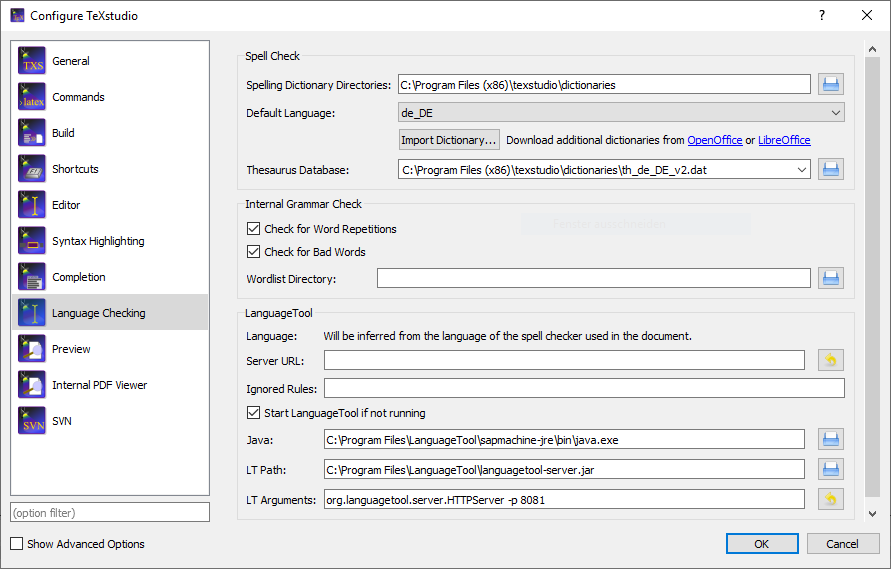
\includegraphics[width=0.9\linewidth]{example_images/texstudio-languagetool-integration}
	\caption[Settings for integrating LanguageTool with TexStudio on ISW computers]{}
	\label{fig:texstudio-languagetool-integration}
\end{figure}

\section{Version control}
\label{sec:version_control}
Whenever working on a document, it is desirable to have some sort of version control. For this task, \ac{ISW} provides a gitlab server found at \url{https://git.isw.uni-stuttgart.de/}. Once you are logged in to gitlab, you can create your own repository for tracking your thesis files. A \texttt{.gitignore} file is necessary to not track all changes to automatically generated files. You may use the \texttt{.gitignore} provided by this template. Again, if \texttt{git} is not installed on your \ac{ISW}-machine, you can install it using OPSI software-on-demand.

You can achieve a rudimentary integration with TeXstudio by defining macros such as the git commit macro shown in \autoref{lst:git_commit}. Note that macros can also be called by using shortcuts.

\begin{lstlisting}[caption={\texttt{git commit} macro}, label={lst:git_commit}]
%SCRIPT
dialog = new UniversalInputDialog()
dialog.setWindowTitle("Git commit")
dialog.add("", "Message", "comment")
dialog.add(false, "Commit all files","allfiles")
if (dialog.exec() != null) {
comment = dialog.get("comment")
if ((dialog.get("allfiles")) == true){
buildManager.runCommand(
"git commit -a -m \"" + comment + "\"", editor.fileName())
}else{
buildManager.runCommand(
"git commit " + editor.fileName() + " -m \"" + comment +
"\"", editor.fileName())
}
}
\end{lstlisting}
